% Shared standalone design for the editable figure reconstructions.
\documentclass[tikz,border=5pt,10pt]{standalone}
\usepackage[T1]{fontenc}
\usepackage[utf8]{inputenc}
\usepackage{newpxtext,newpxmath}
\usepackage[scaled=.94]{sourcesanspro}
\usepackage{pgfplots}
\pgfplotsset{compat=1.18}
\usetikzlibrary{arrows.meta,calc,positioning,decorations.pathreplacing,
  decorations.markings,patterns,matrix,shapes.geometric,fit,backgrounds,
  intersections,angles,quotes}
\definecolor{ink}{HTML}{203746}
\definecolor{accent}{HTML}{146C78}
\definecolor{muted}{HTML}{667780}
\definecolor{signalred}{HTML}{B94B44}
\color{ink}
\tikzset{>=Latex,line width=.8pt,
  every node/.style={font=\small},
  axis/.style={->,draw=muted,line width=.5pt},
  guide/.style={draw=muted,dashed,line width=.45pt},
  curve/.style={draw=accent,line width=1pt},
  marker/.style={circle,fill=accent,inner sep=1.5pt},
  labelbox/.style={fill=white,inner sep=2pt}}

\begin{document}
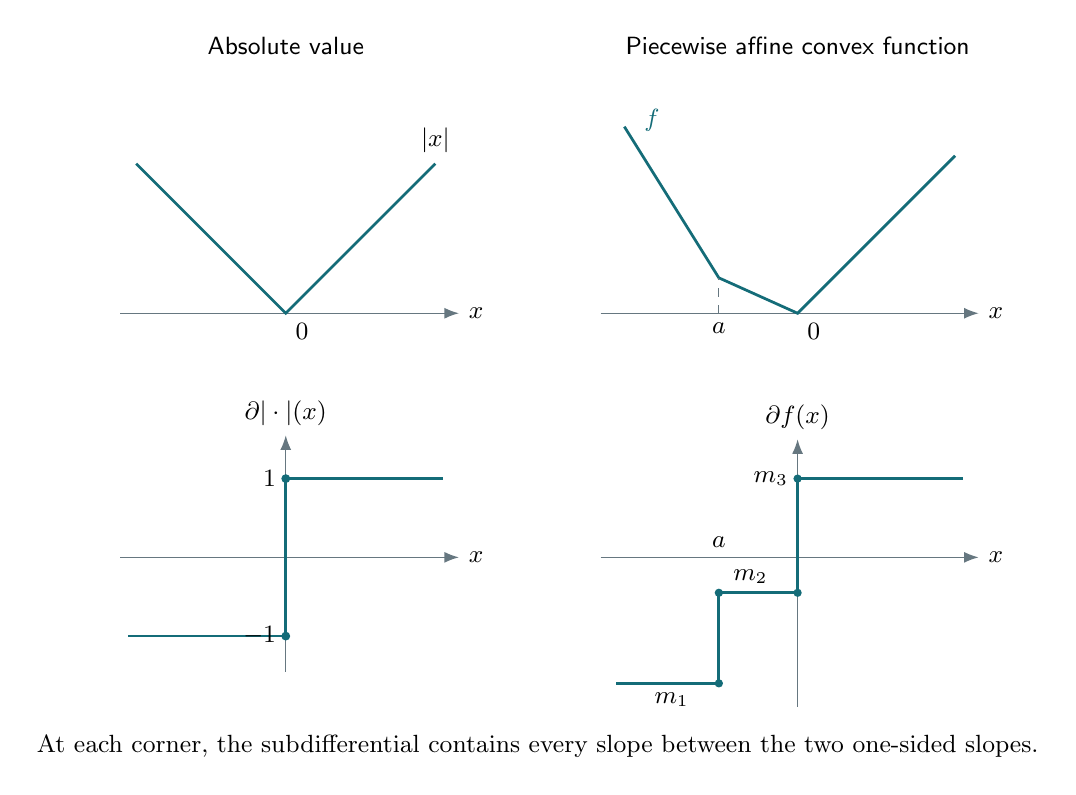
\begin{tikzpicture}
\begin{scope}
\node[font=\small\sffamily]at(0,3.4){Absolute value};
\draw[axis](-2.1,0)--(2.2,0)node[right]{$x$};\draw[curve](-1.9,1.9)--(0,0)--(1.9,1.9)node[above]{$|x|$};
\node[below right]at(0,0){$0$};
\begin{scope}[shift={(0,-3.1)}]
\draw[axis](-2.1,0)--(2.2,0)node[right]{$x$};\draw[axis](0,-1.45)--(0,1.55)node[above]{$\partial|\cdot|(x)$};
\draw[curve](-2,-1)--(0,-1)--(0,1)--(2,1);
\foreach \y in {-1,1}{\fill[accent](0,\y)circle(1.6pt);\node[left]at(0,\y){$\y$};}
\end{scope}
\end{scope}
\begin{scope}[shift={(6.5,0)}]
\node[font=\small\sffamily]at(0,3.4){Piecewise affine convex function};
\draw[axis](-2.5,0)--(2.3,0)node[right]{$x$};
\draw[curve](-2.2,2.37)--(-1,.45)--(0,0)--(2,2);
\draw[guide](-1,0)node[below]{$a$}--(-1,.45);\node[below right]at(0,0){$0$};
\node[accent]at(-1.85,2.45){$f$};
\begin{scope}[shift={(0,-3.1)}]
\draw[axis](-2.5,0)--(2.3,0)node[right]{$x$};\draw[axis](0,-1.9)--(0,1.5)node[above]{$\partial f(x)$};
\draw[curve](-2.3,-1.6)--(-1,-1.6)--(-1,-.45)--(0,-.45)--(0,1)--(2.1,1);
\foreach \x/\y in {-1/-1.6,-1/-.45,0/-.45,0/1}{\fill[accent](\x,\y)circle(1.5pt);}
\node[below]at(-1.6,-1.6){$m_1$};\node[above]at(-.6,-.45){$m_2$};\node[left]at(0,1){$m_3$};
\node[above]at(-1,0){$a$};
\end{scope}
\end{scope}
\node at(3.2,-5.5){At each corner, the subdifferential contains every slope between the two one-sided slopes.};
\end{tikzpicture}
\end{document}
